\section{Experiments}

We have implemented our method in python, using a linkage-matrix\todo{cite,
maybe from the scipy docs} based
data structure to store the tree, and have precomputed and cached several
operations that may need to be repeated every refinement iteration. This allows
us to quickly perform the merge and split operations and calculate the
scores, \dmcmt{TODO ref earlier sections} without having to do (relatively)
expensive tree traversal operations in each iteration of the abstraction
refinement loop. 

Using this implementation, we have performed three sets of experiments to
demonstrate the usefulness of our benchmarks. We first use our abstractions to
attempt to verify safety properties of the \acasxu networks, where we
show that we are able to obtain smaller abstract networks that are sufficiently
strong to verify safety properties. However, abstractions may be useful in other
domains as well, \dmcmt{What? Check Jan Kretinsky, cite}, in particular to
obtain compressed networks with certain safety guarantees behind them. To
demonstrate this, we use our implementation to compress networks trained on the
MNIST networks in the second and third set of experiments. \dmcmt{This needs to
intro our story better}

\dmcmt{TODO add gh link and exp machine details}

\subsection{\acasxu}
\dmcmt{These set of experiments still needs to be rerun}

In these set of experiments, we have taken the \acasxu set of
networks \todo{add detailed table} and
properties and attempt to verify them using a CEGAR approach. We use our
technique to generate the abstraction, and attempt to verify the property on the
abstract network using an existing neural network verification solver. If the
solver returns a counterexample, and if that counterexample is not spurious, we
use that counterexample as a reference point for score calculation \todo{Ref
prev sec} to select the culprit neuron. \todo{Ref prev section} With the culprit
neuron selected, we then refine the network.

\begin{table}
\begin{tabular}{ |c|c|c|c| }
\hline
Benchmarks &    \% Verified &  Avg Reduction &  Avg Time \\
\hline
safe       &        40.404  &         4.4875 &   14.198  \\
unsafe     &       100      &        55.6071 &   12.7916 \\
\hline
\end{tabular}
\caption{Summary of \acasxu Results\todo{Fix formatting}}
\label{t:acas-summary}
\end{table}

The results are summarised in table \ref{t:acas-summary}. The solver we used was
\abcrown. \dmcmt{Note, avg time and network size here doesn't include
timeouts. Also, for reduction rate, the original network size is taken to be
600, since the re-merging optimization is not there in this data. With that
optimization added, we should compare against 300. Also, the full verification
rate is 100\% because its not a full set of experiments, this will potentially
be a lot lower.} 

We notice that for the unsafe cases, we are able to refute the
properties via a counterexample obtained on a significantly smaller network.
\dmcmt{But what about the safe cases, what do we say?}. In fact, for most
networks, we are able to refute based on a counterexample from the fully
abstracted network of size $18$. \dmcmt{This is not there in this small summary
table, but is clear from the full data table. Maybe link to that somewhere
in the appendix?} Note that since we use only two classes in our
fully abstracted network as opposed to 4 in \cite{cegar-nn}, the size of this
network is significantly smaller. In other networks, we are are able to get a
counterexample on a network with size very close to the original network.

For the safe cases, we see that the size of the abstracted networks are large
for instances that did not time out.  This is in line with what was observed in
\cite{cegar-nn} \dmcmt{Can we claim this? It's not immediately clear from their
paper, maybe we need to show our recreation of their experiments? Also, this
split is not clear from the table}. For other instances, the timeout happened
due to the solver timing out on the abstract query. \dmcmt{While the sizes of
the networks on which this to happened are small, does that not say
something negative about our abstraction?}

\begin{figure}
    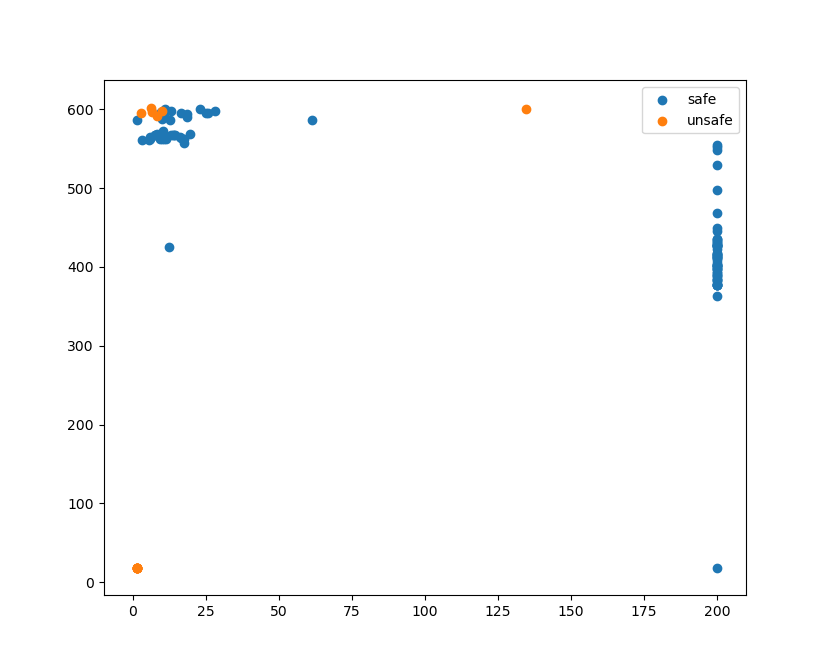
\includegraphics[scale=0.4]{figs/acas-scatter.png}
   \caption{Scatter plot of abstract network sizes vs time in seconds for
   \acasxu}
   \label{f:acas-scatter}
\end{figure}

Figure \ref{f:acas-scatter} shows the network sizes and times of the \acasxu
networks as a scatter plot. \dmcmt{This includes to and non-to}. Note that the
time taken here is dominated by the solver call time \dmcmt{Should we measure
and report this precisely?} We see that the time taken by the solver call on
these networks is not at all correlated with the network sizes. For instances,
for the safe cases, there are several networks of sizes ranging from $350$ to
$600$ \relu nodes all of which time out on the solver call. Similarly, for the
unsafe networks, several $600$ size networks take less than $25$ seconds. In
fact, we found that the time taken by the solver call on a particular network is
more dependent on the solver (and configuration of the solver) used than on the
size of the network. Due to this, in the following experiments, we measure the
accuracy of the networks obtained via abstraction instead of making solver calls
to determine the effectiveness of the abstraction. \dmcmt{Is this okay? Can it
be instead argued that the variance is due to the networks themselves, so the
abstraction is not necessarily useful?
Maybe trying with other configs and showing the variance?}

\subsection{Robustness on \mnist}
\dmcmt{What about doing these experiments on ACAS?}
\dmcmt{Do pgd then samples}

In this section, we start with our abstraction and progressively refine it using
our refinement technique, measuring the number of spurious counterexamples at
each step. To perform the refinement at each step, we try four methods to
perform the culprit neuron selection. The first method 'random' simply chooses a
culprit at random, and serves as a baseline. For the other three methods, we
choose a number of reference points to calculate scores, and choose the culprit
neuron with the highest score. For 'samples', the reference points are random
generated input points that satisfy the precondition. For 'pgd', the samples are
generated via a PGD \todo{cite} attack on the abstract network at each step. For
'samples-pgd', we do some initial refinement steps using the randomly generated
samples, when all the samples have been exhausted, we then perform 'pgd'. We use
the implementation of 'pgd' inside \abcrown for our experiments.

\begin{figure}
    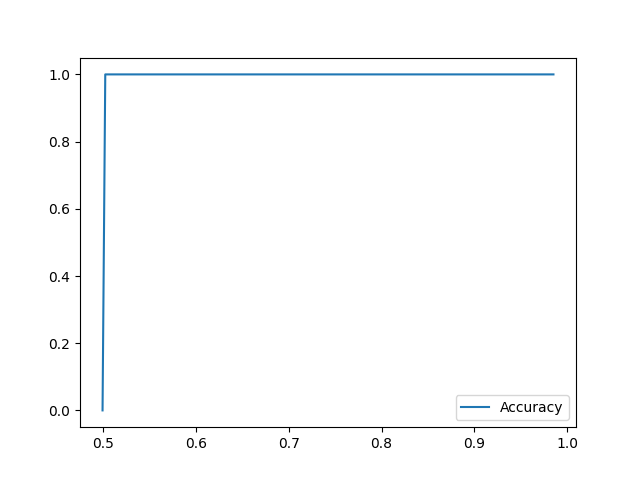
\includegraphics[scale=0.4]{figs/mnist_2_256_prop_0_0.03_samples.png}
    \caption{Accuracy vs Reduction Rate plot for \mnist of size $2 \times 256$
        with $\epsilon$-Robustness property. Refinement done via the 'samples'
    method.}
    \label{f:mnist-prop-samples}
\end{figure}
\begin{figure}
    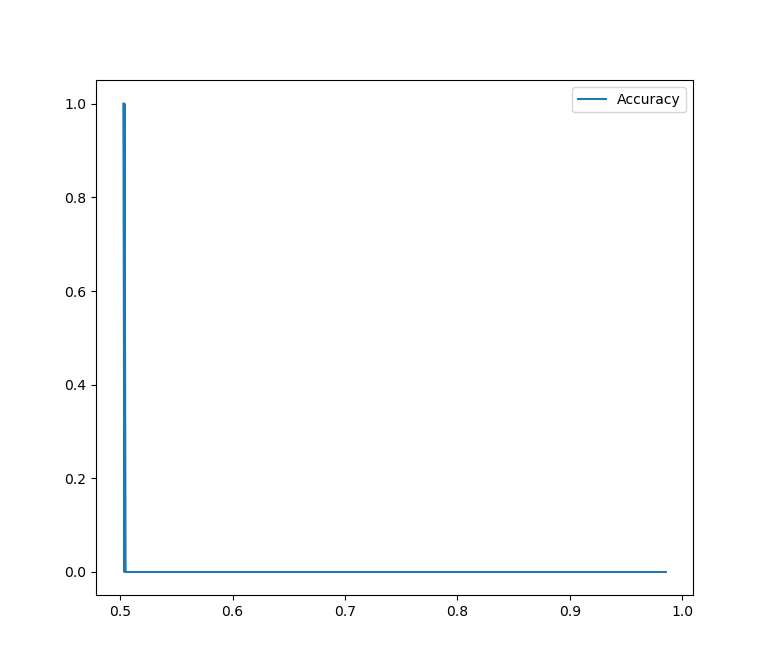
\includegraphics[scale=0.4]{figs/mnist_2_256_prop_0_0.03_pgd.png}
    \caption{Accuracy vs Reduction Rate plot for \mnist of size $2 \times 256$
        with $\epsilon$-Robustness property. Refinement done via the 'pgd'
    method.}
    \label{f:mnist-prop-pgd}
\end{figure}

Figure \ref{f:mnist-prop-samples} \ref{f:mnist-prop-pgd} shows a typical plot
for these experiments.  Here accuracy measures the number of true
counterexamples within a random sample
drawn from a region satisfying the pre-condition. \dmcmt{Should I plot and talk
in terms or spurious counterexample rate instead?} We see that as we refine the
network and the reduction rate reduces (moving right to left along the graph),
the accuracy remains close to zero. At some point however, the accuracy jumps up
sharply and becomes close to $100\%$. This indicates that there are a few
critical refinement steps that remove almost all spurious counterexamples. This
may be due the fact that with epsilon robustness properties that are being
explored here, the pre-condition region may be very small, so a single
refinement step may change the behavior of the network on that small region in a
way that eliminates all possible spurious counterexamples from that region.
\dmcmt{Is this expl okay?}
\dmcmt{BaB and abstract interp based methods like \abcrown are successful on
such props because of this, discuss this?} \dmcmt{Also, other graphs are
present. For eg, some random sampling graphs show peaks in the middle
(2..random), and some pgd graphs are flat lines (4,6..pgd). Discuss
these?}

\begin{table}
\begin{tabular}{|c|c|c|c|c|}
    \hline
    Net Size     & Cex Method  & Reduction & Accuracy & No. Steps \\
    \hline
    $2\times256$ & random      & $49.1\%$  & $100\%$  & $ 809$    \\
    $4\times256$ & random      & $49.6\%$  & $100\%$  & $1778$    \\
    $6\times256$ & random      & $49.7\%$  & $100\%$  & $2602$    \\
    $2\times256$ & samples     & $50.3\%$  & $100\%$  & $  27$    \\
    $4\times256$ & samples     & $49.9\%$  & $100\%$  & $ 648$    \\
    $6\times256$ & samples     & $47.9\%$  & $100\%$  & $1199$    \\
    $2\times256$ & pgd         & $50.4\%$  & $100\%$  & $  28$    \\
    $4\times256$ & pgd         & $88.6\%$  & $  0\%$  & $  14$    \\
    $6\times256$ & pgd         & $83.3\%$  & $  0\%$  & $  82$    \\
    $2\times256$ & samples-pgd & $50.3\%$  & $100\%$  & $  27$    \\
    $4\times256$ & samples-pgd & $49.9\%$  & $100\%$  & $ 648$    \\
    $6\times256$ & samples-pgd & $47.9\%$  & $100\%$  & $1209$    \\
    \hline
\end{tabular}
\caption{Summary of \mnist Results on a single robustness property \todo{Fix
formatting} \dmcmt{Include Times?}}
\label{t:mnist-prop-summary}
\end{table}

Table \ref{t:mnist-prop-summary} summarizes these results for multiple \mnist
networks and multiple refinement methods. Accuracy here refers to the final
accuracy of the best network found when the refinement process stops due to lack
of counterexamples. We find that 'pgd' performs poorly on the $4$ and $6$ layer
networks, where while the number of steps are relatively low and the reduction
rate is high, the accuracy is very low. This is because the \abcrown
implementation of \pgd fails to find a spurious counterexample early on in the
refinement process for these instances, leading to early termination without
ever hitting the accuracy jump. The 'random' method performs consistently worse
than the others in terms of the number of steps. Apart from these exceptions,
the other instances and methods seem to perform comparably on the same network.
We may conclude two things from this data. Firstly, although the 'pgd' method
incurs a significant time overhead \dmcmt{Measure?} it does not necessarily
provide any benefits. Secondly, we are able to follow our refinement process
to obtain a satisfactory compression of the network with a very low probability
of finding a spurious counterexample, which is evidence towards our hypothesis
that a satisfactory abstraction exists within the restricted search space
defined via our tree.
